\chapter{Multipath TCP}
\label{chap:multipathtcp}

\section{Transmission Control Protocol (TCP)}
MPTCP is an extension of regular TCP, the ubiquitous protocol for highly reliable host-to-host communication in a packet-switched computer network. A proper introduction of the fundamental of TCP is due.


The reasons why TCP became a de-facto standard in modern computer communication has been briefly mentioned in the introductory part of the paper. A more technical analysis shows that TCP maintains good levels of reliability for the connection independently from the lower layers it depends on for the raw transmission of bits. TCP is indeed able to handle possible data loss, data damaging, data duplication, out of order delivery of data. In order to do this, the data to be transmitted is split into a sequence of TCP packets, each containing an additional \textit{TCP header} with the information needed to operate the protocol functionalities at the nodes. Such functionalities are [\href{https://tools.ietf.org/html/rfc793}{ref}]:

\begin{itemize}
  \item \textit{Basic data transfer}: sending continuous stream of octets in each direction between its users, identified by the 4-tuple: source IP address, source port, destination IP address, destination port. The IP address allows to route packets to the destination machines, while the port values direct the content of the packet to the right application within a host;
  \item \textit{Reliability}: in-order, reliable data transfer is achieved by adding a sequence number to each transmitted octet and using ACK signals and timeouts to possibly trigger retransmission of lost packets. TCP assures that no transmission errors will affect the delivery of the data if the network is not completely partitioned;
  \item \textit{Flow control}: the receiver can control the amount of data sent by the sender in a certain moment of the connection by returning a "window" value in the TCP header, so that it is possible to avoid buffer congestion;
  \item \textit{Multiplexing}: a single host is allowed to use multiple independent TCP connections simultaneously thanks to the port value available in the protocol. This value, together with the host address assigned at the internet communication layer, forms a socket, that is the actual endpoint of a TCP connection;
  \item \textit{Connections}: TCP initializes and maintains status information regarding each connection and the data stream between a pair of sockets in order to provide all its functionalities. Such status information is initialized during a first handshake procedure, and released only upon connection termination. TCP is indeed known as a virtual-connection protocol;
  \item \textit{Precedence and Security}: these aspects refer to the possibility of prioritize connections and assign security properties to them. Both precedence and security can be configured by users, but default values are provided.
\end{itemize}

As noted above, all these features are made possible by processing the bits at the TCP header. Such structured set of information is mostly static and predefined, so that at each position in the header corresponds a well known portion of the protocol data. The TCP header looks like the one in Figure \ref{fig:tcp_header}.

\begin{figure}[!htb]
\centering
\includegraphics[width=0.75\textwidth]{images/tcp_header}
\caption{The TCP header format}
\label{fig:tcp_header}
\end{figure}

The \textit{Source Port} and \textit{Destination Port}, together with the source and destination IP addresses provided in the upper IP header (not shown in figure \ref{fig:tcp_header}), are the means for identifying the two endpoints of the TCP connection. \textbf{These static fields clearly shows the single-path fundamental design of the protocol}. 


TCP assures reliability standards independently from the lower layers used to route packets and transmit raw bits, and it is possible that packets arrive at destination unordered, or that some of them are lost on the way: \textit{Sequence Number}, \textit{Acknowledgment Number} and \textit{Data Offset} are three fields used in TCP for such cases; numbering each octet it is possible to put them in sequence and acknowledge them in a cumulative way, so that by acknowledging sequence number X means that all packets up to but not including X has been received. This system, together with timeouts, allows for retransmission of lost packets.
Other interesting fields in the header are: the \textit{Window} field, which allows to achieve congestion control by telling to the sender the range of sequence numbers the data receiver is prepared to accept in a particular instance of time; the \textit{Checksum} field guarantees that data has not been modified on its way to the destination, intentionally or unintentionally (thus being part of the reliability aspect of the protocol).


A component of the TCP header that is fundamental for MPTCP is the \textit{Options} field, which was firstly introduced as a free space for future additions to the protocol. In this specific case, the TLV solution is adopted to process the data inside the field. "TLV" stands for \textit{type-length-value}, where the type is the ID value uniquely identifying the option, the length is the number of bytes of the option, whereas the value represents the actual option content. This particular design allows to skip unknown options at the receiver by simply checking the length value and moving the pointer accordingly. An important limitation for this field is that its total length cannot be more than 40 bytes [ref].

\section{MPTCP design}
MPTCP \textit{functional goals} are to increase resilience of the connectivity and efficiency of the resource usage.
Such goals can be found very similar in other multipathing solutions as the ones described in section [add section], but what is really unique about MPTCP protocol design is the set of its \textit{compatibilities goals} [\href{https://tools.ietf.org/html/rfc6182}{ref}]:

\begin{itemize}
  \item \textit{Application compatibility} aims at instantiating a protocol that can be fully operational with no modifications for the applications using it. This means that the networking APIs and the overall service model of regular TCP has to be maintained with MPTCP; the entire MPTCP functioning is handled transparently by the underlying system. Such transparency must be maintained also in terms of throughput, resilience and security for the connection, that cannot be deteriorated with respect to the current TCP standards;
  \item \textit{Network compatibility} is a goal similar to the previous one, since MPTCP is supposed to work out of the box with the current underlying network layer and the ones below it. The main reason still resides in the possibility of achieving a smooth wide-spread deployment of the protocol on the current infrastructure;
  \item \textit{Users compatibility} is a corollary to both network and application compatibility, which states that MPTCP flows must be fair to regular TCP connection in case of shard bottlenecks.
\end{itemize}


All these compatibilities requirements should explain the very fundamental decision of developing the new multipath protocol at the transport layer, and more specifically as an extension of regular TCP. Let's take into consideration the traditional TCP protocol stack and compare it to the new MPTCP stack (figure \ref{fig:stack});

\begin{figure}[!htb]
\centering
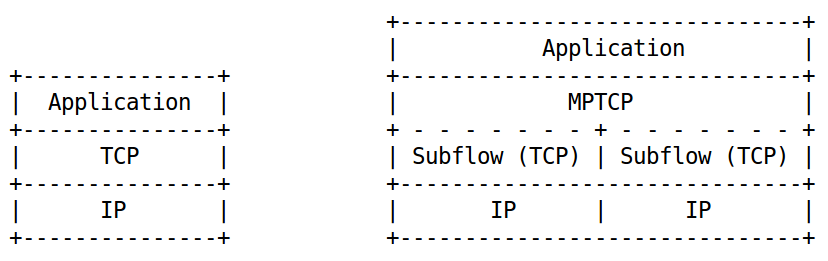
\includegraphics[width=0.75\textwidth]{images/stack}
\caption{The TCP and MPTCP protocol stacks}
\label{fig:stack}
\end{figure}

To achieve the required compatibility goals, changes had to be applied to layers lower than the application layer, so that current programs do not have to be upgraded to make use of multipath; on the other side, the new protocol had to be placed at layers above the network layer, which is the last layer still operating at the network infrastructure before the transport layer, the latter being the first layer operating at the end systems. The idea with MPTCP is to deploy it as a simple upgrade of the end systems' OS, with no modifications applied to the network infrastructure.


The choice of working at the transport layer was indeed the only available option. Within that option, the choice of maintaining TCP as the fundamental operating protocol for MPTCP was still straightforward for similar compatibility reasons; for this very purpose engineers decided to add all the required options for MPTCP inside the TCP \textit{Option} field in the TCP header. In this way, MPTCP-aware systems can process the MPTCP options for multipathing, but if a system that is not MPTCP-aware receives a MPTCP connection-request, it would simply discard the MPTCP options and threat such message as a plain TCP connection-request. 
MPTCP design maintains the behavior of the subflows to be compliant with regular TCP, while reassembling of data incoming from different paths is a process executed by the receiving host only. MPTCP subflows are indeed seen by middleboxes as regular and independent TCP connections carrying additional options. If security policies at the middleboxes is not too restrictive against unknown options, MPTCP-unaware nodes would still work with the new protocol.
For what regards applications, they don't need to be changed either since MPTCP would be inserted into the network stack at the operating system level: it would automatically split the data buffered from the application layer and send it through different subflows, according to the number of available endpoints at the connected hosts. Communication with the application layer can be performed through the old TCP APIs, even if MPTCP specific options can be used by upgraded user programs to take advantage of more advanced options in MPTCP.


It should be now clear that the core implementation of MPTCP rotates around a relatively compact set of TCP options. Technically, there is only a single generic MPTCP option, to which has been assigned the value 30 as the "Kind" identifier; at a lower level it is possible to identify a set of eight MPTCP option subtypes, each identified by a 4 bit value (\ref{fig:MPTCP_options}).

\begin{figure}[!htb]
\centering
\includegraphics[width=0.75\textwidth]{images/MPTCP_options}
\caption{The set of MPTCP options}
\label{fig:MPTCP_options}
\end{figure}

All of these options are used to implement the entire behavior of MPTCP, mainly handling subflow sessions (control plane) and handling the data transfer within a single session (data plane).

\subsection{Control plane}
\subsubsection{MP\_CAPABLE}
The connection initiation of an MPTCP connection is very similar to the standard TCP initial handshake, involving a SYN, SYN/ACK and ACK exchange on a single path between host A and host B. At the TCP level, with the exchange of such three packets both hosts have received an acknowledgment of the connection and they also have exchanged the two random sequence numbers that will be used for the two directions of the connection.
In the MPTCP case, the SYN packet from host A will have a MP\_CAPABLE option in the \textit{Options} field of the TCP header; apart from that, the rest of the packet behaves exactly as in regular TCP: in fact, if the receiver host B is not MPTCP-compatible it will simply discard the MP\_CAPABLE option and instantiate a regular TCP connection.
In case both hosts are MPTCP-compatible, the MP\_CAPABLE option is inserted in the three packets of the initial handshake for two purposes: advertise that both hosts are indeed MPTCP-compatible and allow them to exchange two 64-bit keys, according to the scheme in figure \ref{fig:mpcapable}.

\begin{figure}[!htb]
\centering
\includegraphics[width=0.75\textwidth]{images/mpcapable}
\caption{MPTCP connection initiation}
\label{fig:mpcapable}
\end{figure}

These keys are sent in clear inside the MP\_CAPABLE option only during the initial handshake and their purpose is to identify a specific MPTCP connection within a host (useful when associating a new subflow to an existing MPTCP connection for example) and to provide shared security material that is used in MPTCP for authorization mechanisms (more on this later in this section). The \textit{Option} field in the TCP header can only be 40 bytes long, and it is not reserved to MPTCP only. For this reason it is of primary importance to keep the amount of MPTCP related metadata as low as possible. In fact, the original 64 bit keys are exchanged only during initial handshake; subsequently, shorter 32 bit tokens derived from such keys will be used to address a specific MPTCP connection, even if this procedure requires additional checks in case of collisions with other tokens already assigned to other MPTCP connections in the same machine.

\subsubsection{MP\_JOIN}
Suppose that after the first subflow is operational, host A initiates a new subflow between one of its addresses and one of host B's addresses (figure \ref{fig:mpjoin}). Host A sends a TCP packet to host B containing the MP\_JOIN option, which includes Token-B (the token derived B's key) and a nonce value used to prevent replay attacks. An additional field in the MP\_JOIN option is called Address ID, an identifier for the original addresses in use within a single MPTCP connection; this additional value allows to refer to a well known subflow without the need to check the addresses, which is very useful when middleboxes like NATs alter the IP header during the transit of the packets.

\begin{figure}[!htb]
\centering
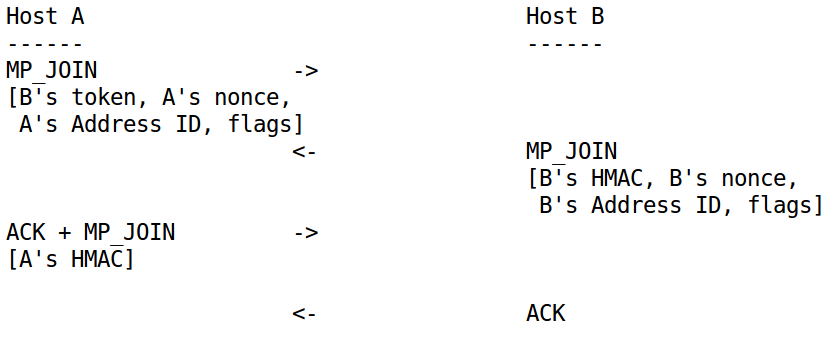
\includegraphics[width=0.75\textwidth]{images/mpjoin}
\caption{MPTCP additional subflows}
\label{fig:mpjoin}
\end{figure}

\subsection{Data plane}
This part concerns all the MPTCP options used to manage the data flow in a MPTCP connection, including how the byte stream is subdivided into different subflow and how the original order of the packets is provided at the receiver.

\section{MPTCP deployment}
After having explained all the technicalities about the protocol, it is now possible to talk about its deployment status and the problems encountered by pairing MPTCP with current infrastructures. This might seem a bit outside the scope of the thesis, but it is worth mentioning that the \textit{deployment status} and \textit{implementations} are a good indicator of how much MPTCP is important in the Internet community and they are good topics to motivate the thesis work. Also \textit{middleboxes compatibility} is indeed a fundamental part of the MPTCP security evaluation, being monitoring and detection equipment part of these middleboxes.

\subsection{Middleboxes compatibility}
This section will be quite technical and it is supposed to list the most important middle-boxes and their impact/effect on a MPTCP connection. These boxes include NATs, proxies and firewalls. This part should clearly state why MPTCP widespread adoption is a big challenge.

\subsection{Implementations}
Despite the previously described problematics, MPTCP is a big bet in the IETF community and many implementations have been developed for the most common OSes, listed in this section (with some history notions).

\subsection{Deployment status}
It should be interesting for the reader to go through some examples of real world's scenarios in which MPTCP is used successfully. Here it is possible to cite some important achievements related to MPTCP (for example the highest throughput ever reached with the new protocol).
If available, it would be also good to show some graphs about MPTCP adoption rate or similar.